% =======================================================
% 5. RESOCONTO ATTIVITA' DI VERIFICA
% =======================================================
\section{Resoconto Attività di Verifica}
In questa sezione vengono riportati i risultati delle attività di verifica condotte durante la fase di RTB. L'obiettivo è fornire una panoramica oggettiva del livello di qualità raggiunto.

\subsection{Verifica documentazione}
La verifica della documentazione (Analisi dei Requisiti, Norme di Progetto, Piano di Progetto, Verbali e Glossario) è avvenuta tramite revisione manuale incrociata. Il Verificatore\textsubscript{G} ha controllato la coerenza dei contenuti, l'assenza di errori grammaticali e il rispetto degli standard di formattazione definiti nelle \link{https://synergo-unit-unipd.github.io/Second-Brain/docs/PB/doc_gestionali/doc_interni/norme_di_progetto/norme_di_progetto.pdf}{Norme di Progetto}.
\\ \\
Tutti i documenti pubblicati hanno superato il controllo di qualità, raggiungendo un indice di leggibilità conforme ai parametri accettabili.

\subsection{Verifica codice}
A partire dalla fase PB, la verifica del codice includerà test automatizzati eseguiti con pytest per il backend
 e vitest per il frontend e controlli di qualità statica tramite eslint e prettier. Tali strumenti saranno
 integrati nella pipeline di CI per garantire il rispetto delle soglie di copertura e delle regole di stile.

\subsection{Copertura test}
Durante la RTB, la copertura riguarda esclusivamente la tracciabilità tra i Casi d'Uso e i Test di Sistema definiti nella sezione precedente. Il 100\% degli UC individuati è stato coperto da almeno un Test di Sistema (stato NI).

\subsection{Esiti test}
Allo stato attuale, non sono stati eseguiti test dinamici sul software. Gli unici esiti riguardano le ispezioni documentali, che hanno evidenziato una progressiva riduzione dei difetti formali grazie all'affinamento delle modalità di verifica.

\newpage
% =======================================================
% 6. VALUTAZIONI PER IL MIGLIORAMENTO
% =======================================================
\section{Valutazioni per il Miglioramento}
Il gruppo Synergo Unit adotta il metodo \textbf{PDCA} (Plan-Do-Check-Act) per garantire il miglioramento continuo dei processi.

\subsection{Retrospettive}
Al termine di ogni Sprint, il gruppo si riunisce per analizzare cosa ha funzionato e cosa può essere ottimizzato. Durante la RTB, è emersa la necessità di automatizzare maggiormente la compilazione di alcune tabelle LaTeX per ridurre il tempo di verifica manuale.

\subsection{Azioni correttive}
A fronte di anomalie rilevate dalle metriche o durante le revisioni, sono state stabilite le seguenti contromisure:

\begin{table}[H]
    \centering
    \renewcommand{\arraystretch}{1.3}
    \begin{tabularx}{\textwidth}{|p{6cm}|p{6.5cm}|X|}
        \hline
        \rowcolor{primarycolor!10}
        \textbf{Problema Rilevato} & \textbf{Contromisura Adottata} & \textbf{Rischio correlato} \\
        \hline
        Difficoltà iniziale nella gestione della sintassi LaTeX complessa. & Creazione di un repository di template\textsubscript{G} condivisi per tabelle e strutture ricorrenti. & RT1 \\
        \hline
        Incoerenza nella numerazione dei Casi d'Uso (UC) tra diversi documenti. & Revisione centralizzata dell'Analisi dei Requisiti e allineamento immediato dei test. & RR1, RO5 \\
        \hline
        Frequenti conflitti durante l'unione del codice sorgente (merge conflicts). & Utilizzo sistematico di un repository GitHub e adozione di un workflow basato su branch\textsubscript{G} per isolare le funzionalità. & RT4 \\
        \hline
        Difficoltà nel tracciamento puntuale delle attività (task) e delle ore spese dai singoli membri. & Utilizzo di GitHub Projects e GitHub Issues per l'assegnazione dei compiti e il monitoraggio dello stato di avanzamento (ToDo, In Progress, In Review, Done). & RO3 \\
        \hline
        Eccessivo carico burocratico e rischio di errore umano nella creazione manuale dei task e nella raccolta dati. & Automazione del processo tramite un form dedicato per la generazione automatica delle Issue. I dati vengono centralizzati in un foglio di calcolo\textsubscript{G} per la generazione automatica della rendicontazione e del cruscotto. & RO6, RO7 \\
        \hline
    \end{tabularx}
    \caption{Storico delle azioni correttive}
\end{table}

\subsection{Problemi aperti}
Rimane aperta la questione della selezione del framework\textsubscript{G} di testing definitivo per l'integrazione con le API LLM, che verrà risolta all'inizio della fase PB dopo un'analisi tecnologica approfondita.

\newpage
% =======================================================
% 7. CRUSCOTTO DELLE METRICHE
% =======================================================
\section{Cruscotto delle Metriche}
In questa sezione sono riassunti i valori ottenuti dalle metriche durante l'ultimo Sprint della fase RTB.

\subsection{Stato attuale qualità di processo}
\begin{table}[H]
    \centering
    \renewcommand{\arraystretch}{1.3}
    \begin{tabularx}{\textwidth}{|l|X|c|c|}
        \hline
        \rowcolor{primarycolor!10}
        \textbf{Codice} & \textbf{Nome Metrica} & \textbf{Valore Rilevato} & \textbf{Esito} \\
        \hline
        MPC01 & Schedule Performance Index & 1.05 & Ottimale \\
        \hline
        MPC02 & Cost Performance Index & 0.98 & Accettabile \\
        \hline
        MPC03 & Requirements Stability Index & 85\% & Accettabile \\
        \hline
        MPC04 & Time Efficiency & 75\% & Accettabile \\
        \hline
        MPC05 & Task Completion Rate & 100\% & Ottimale \\
        \hline
        MPC06 & PR Resolution Time & 2 giorni & Accettabile \\
        \hline
        MPC07 & Review Coverage & 100\% & Ottimale \\
        \hline
        MPC08 & Quality Metrics Compliance Rate & 100\% & Ottimale \\
        \hline
    \end{tabularx}
    \caption{Riepilogo Qualità di Processo}
\end{table}

\subsection{Stato attuale qualità di prodotto}
\begin{table}[H]
    \centering
    \renewcommand{\arraystretch}{1.3}
    \begin{tabularx}{\textwidth}{|l|X|c|c|}
        \hline
        \rowcolor{primarycolor!10}
        \textbf{Codice} & \textbf{Nome Metrica} & \textbf{Valore Rilevato} & \textbf{Esito} \\
        \hline
        MPD01 & Soddisfacimento Requisiti Obbligatori & 100\% & Ottimale \\
        \hline
        MPD02 & Comment Density & N/D & N/D \\
        \hline
        MPD03 & Browser Compatibility & N/D & N/D \\
        \hline
        MPD04 & Errori Ortografici (per pagina) & 0 & Ottimale \\
        \hline
        MPD05 & Complessità Ciclomatica & N/D & N/D \\
        \hline
        MPD06 & Tempo di Caricamento Iniziale & N/D & N/D \\
        \hline
        MPD07 & Indice di Gulpease (Media Documenti) & 52,62 & Accettabile \\
        \hline
    \end{tabularx}
    \caption{Riepilogo Qualità di Prodotto}
\end{table}
Le metriche MPD02, MPD03, MPD05 e MPD06 sono pianificate per la fase PB, poiché richiedono 
la disponibilità di codice sorgente stabile o di un prodotto eseguibile su cui 
effettuare misurazioni significative.


\subsection{Grafici e dashboard}
L'andamento storico delle metriche viene monitorato tramite grafici temporali per evidenziare eventuali trend negativi.

\subsubsection{Trend di Progetto}
 \begin{figure}[H]
	    \centering
	    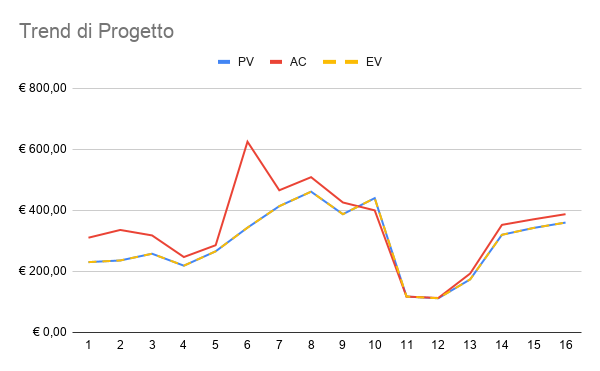
\includegraphics[width=0.8\textwidth]{grafici/trend.png}
	    \caption{Andamento PV\textsubscript{G}, AC\textsubscript{G}, EV\textsubscript{G}}
	 \end{figure}

Il grafico riporta l'andamento cumulato, sprint dopo sprint, del Planned Value\textsubscript{G} (PV), dell'Actual Cost\textsubscript{G} (AC) e dell'Earned Value\textsubscript{G} (EV).

Dal grafico si osserva una perfetta sovrapposizione tra la curva del PV e quella dell'EV lungo tutti i 14 sprint: questo indica che il gruppo è riuscito a completare costantemente il 100\% del lavoro pianificato per ogni iterazione, rispettando in pieno le tempistiche previste.

Analizzando l'Actual Cost (AC), dopo la fase di rientro del debito maturata tra gli sprint 9 e 11, nelle ultime iterazioni si registra un andamento sostanzialmente allineato alle stime, con lievi scostamenti fisiologici dovuti alle attività amministrative, di revisione collaborativa e di setup vari. Nello sprint 13 l'AC si è attestato a 192,92~\euro\ a fronte di un EV di 173,75~\euro, mentre nello sprint 14 l'AC è stato di 352,50~\euro\ contro un EV di 340,00~\euro. L'andamento complessivo dei costi rimane pienamente sotto controllo, con una gestione delle risorse economica e stabile.


\subsubsection{Varianze di Progetto}
 \begin{figure}[H]
	    \centering
	    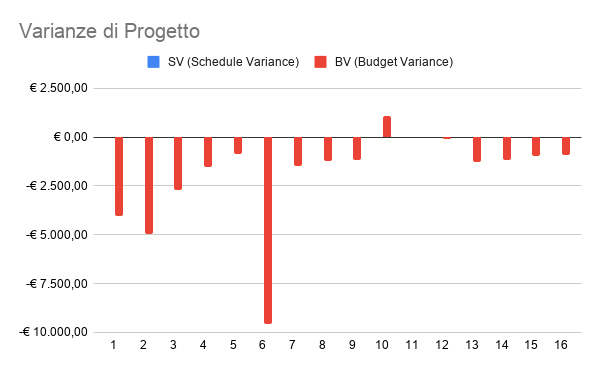
\includegraphics[width=0.8\textwidth]{grafici/varianze.png}
	    \caption{Andamento SV\textsubscript{G}, BV\textsubscript{G}}
	 \end{figure}

Il grafico illustra l'andamento della Schedule Variance\textsubscript{G} (SV) e della Budget Variance\textsubscript{G} (BV).

Coerentemente con quanto osservato nei trend di progetto, la Schedule Variance si mantiene costantemente a 0,00~\euro\ per tutti i 14 sprint: questo è il risultato matematico del perfetto allineamento tra il lavoro completato (EV) e quello pianificato (PV), confermando la totale assenza di ritardi temporali.

Per quanto riguarda la Budget Variance, dopo il marcato avanzo positivo registrato negli sprint 9 e 10, negli sprint 13 e 14 si evidenziano lievi variazioni negative (pari rispettivamente a -19,17~\euro\ nello sprint 13 e -12,50~\euro\ nello sprint 14). Tali scostamenti, dovuti al maggior carico orario richiesto dai ruoli di Amministratore e Verificatore, rientrano ampiamente nelle soglie di tolleranza ammissibili e non compromettono la stabilità economica del progetto, che registra un totale residuo di 6.966,67~\euro.


\subsubsection{Indici di Performance}
 \begin{figure}[H]
	    \centering
	    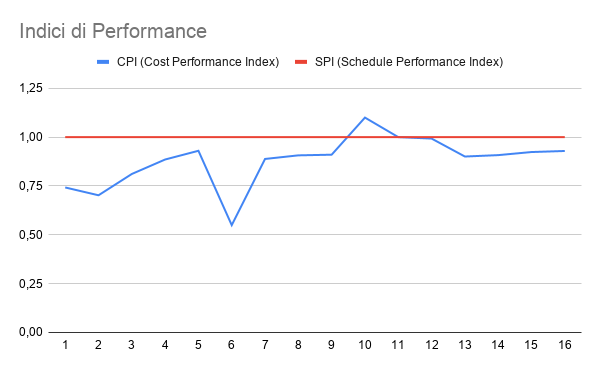
\includegraphics[width=0.8\textwidth]{grafici/performance.png}
	    \caption{Andamento CPI, SPI}
	 \end{figure}

Il grafico riporta l'andamento sprint per sprint del Cost Performance Index (CPI) e dello Schedule Performance Index (SPI). 

Lo SPI si mantiene stabilmente sulla linea ottimale di 1,0 per tutti i 14 sprint conclusi, a dimostrazione di una pianificazione e di un'esecuzione delle tempistiche costantemente prive di ritardi.

Il CPI, dopo essere risalito sopra la soglia ottimale di 1,0 negli sprint 9, 10 e 11, nelle ultime iterazioni si assesta su valori prossimi alla parità (0,90 nello sprint 13 e 0,96 nello sprint 14). La combinazione dei due indici (SPI a 1,0 e CPI stabile attorno all'unità) conferma l'efficienza globale del team sia nel rispetto delle scadenze sia nella gestione del budget allocato.


\subsubsection{Previsione Spesa Finale}
 \begin{figure}[H]
	    \centering
	    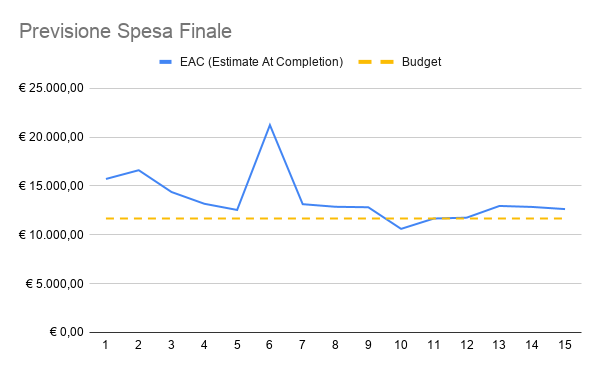
\includegraphics[width=0.8\textwidth]{grafici/previsione_spesa.png}
	    \caption{Andamento EAC\textsubscript{G}}
	 \end{figure}

Il grafico illustra l'andamento dell'Estimate at Completion\textsubscript{G} (EAC). La linea orizzontale tratteggiata rappresenta il BAC\textsubscript{G} (Budget at Completion\textsubscript{G}), fissato a 11.665~\euro.

L'andamento della stima a finire rispecchia l'evoluzione del CPI nel tempo. Superato il picco critico iniziale dello sprint 6 e l'importante fase di recupero culminata negli sprint 9--11, la curva dell'EAC si stabilizza nelle iterazioni 12, 13 e 14 in prossimità della linea del BAC.

Tali dati confermano che il gruppo sta mantenendo la proiezione del costo finale complessivo perfettamente in linea con il budget preventivato, garantendo il completamento delle attività entro i limiti finanziari stabiliti.


\subsubsection{Requisiti}
 \begin{figure}[H]
	    \centering
	    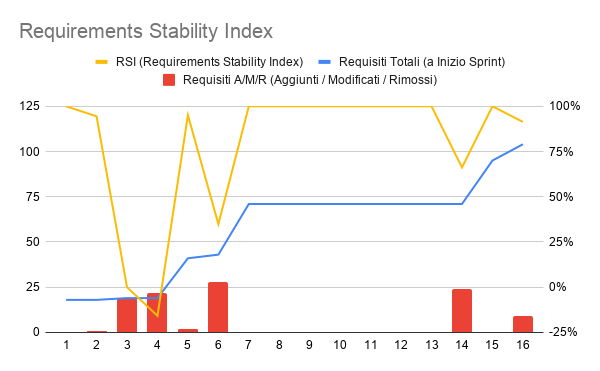
\includegraphics[width=0.8\textwidth]{grafici/RSI.png}
	    \caption{Andamento Requisiti\textsubscript{G}}
	 \end{figure}
Il grafico descrive l'andamento del Requirement Stability Index (RSI) di sprint in sprint.
L'RSI si mantiene stabile nel corso dei vari sprint. Si nota un incremento sostanziale dei requisiti all'inizio degli sprint 5 e 7, in concomitanza con i riscontri ricevuti durante i colloqui con il docente. Negli sprint recenti, compreso lo sprint 14, l'indice evidenzia un'elevata stabilità a seguito del colmamento del gap numerico dei requisiti e del completamento delle tabelle di tracciamento fonti-requisiti.

\subsubsection{Correttezza Ortografica}
 \begin{figure}[H]
	    \centering
	    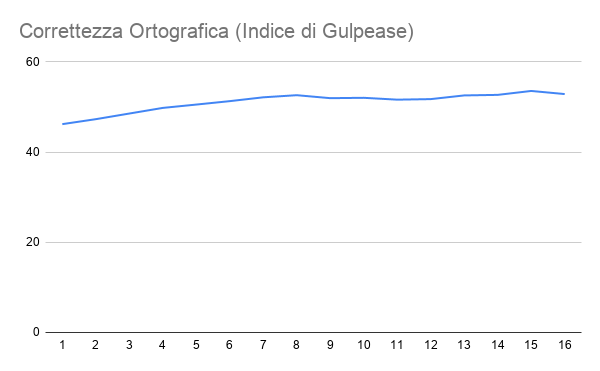
\includegraphics[width=0.8\textwidth]{grafici/gulpease.png}
	    \caption{Indice di Gulpease\textsubscript{G}}
	 \end{figure}
Il grafico illustra l'andamento dell'Indice di Gulpease, utilizzato per monitorare la leggibilità e la chiarezza della documentazione in lingua italiana. 
Nel corso degli sprint si osserva un costante mantenimento di valori compresi nella fascia di accettabilità ($\ge 40$ e $< 80$). Il trend positivo si conferma e si stabilizza negli ultimi sprint raggiungendo l'attuale valore di 55,40. Tale risultato attesta un livello di leggibilità adeguato e una costante attenzione del gruppo alle attività di revisione e verifica editoriale dei documenti.

\subsubsection{Sprint Goal Achievement}
 \begin{figure}[H]
	    \centering
	    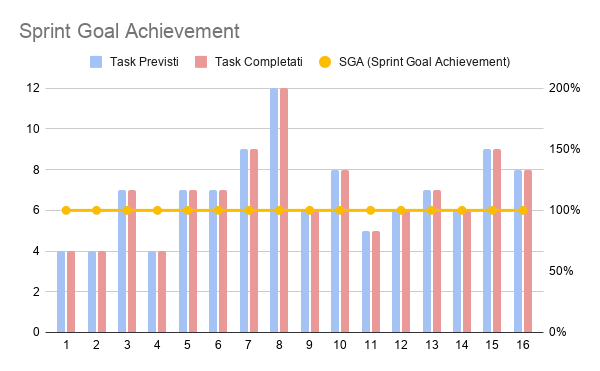
\includegraphics[width=0.8\textwidth]{grafici/task.png}
	    \caption{Andamento task\textsubscript{G}}
	 \end{figure}
Il grafico mostra lo Sprint Goal Achievement (SGA) per osservare il numero di task previste ed effettivamente completate durante i vari sprint. In tutti i 14 sprint svolti finora è stato raggiunto il 100\% di completamento dei task pianificati, confermando la continuità operativa del gruppo e il pieno raggiungimento degli obiettivi stabiliti per ciascun iterazione.